\documentclass[fleqn]{article}
\oddsidemargin 0.0in
\textwidth 6.0in
\thispagestyle{empty}
\usepackage{import}
\usepackage{amsmath}
\usepackage[backend=bibtex]{biblatex}
\usepackage[utf8]{inputenc}
\usepackage{csquotes}
\usepackage{graphicx}
\usepackage{flexisym}
\usepackage{calligra}
\usepackage{amssymb}
\usepackage{bigints} 
\usepackage[english]{babel}
\usepackage{float}
\usepackage[colorinlistoftodos]{todonotes}
\usepackage{blindtext}
\usepackage{hyperref}

\addbibresource{references.bib}

\hypersetup{
  colorlinks=true,
  linkcolor=blue,
  filecolor=magenta,      
  urlcolor=cyan,
  pdfpagemode=FullScreen
}

\DeclareMathAlphabet{\mathcalligra}{T1}{calligra}{m}{n}
\DeclareFontShape{T1}{calligra}{m}{n}{<->s*[2.2]callig15}{}
\newcommand{\scriptr}{\mathcalligra{r}\,}
\newcommand{\boldscriptr}{\pmb{\mathcalligra{r}}\,}


\setlength{\arrayrulewidth}{0.5mm}
\setlength{\tabcolsep}{18pt}
\renewcommand{\arraystretch}{1.5}

\definecolor{hwColor}{HTML}{AD53BA}

\begin{document}

  \begin{titlepage}

    \newcommand{\HRule}{\rule{\linewidth}{0.5mm}}

    \center

    \begin{center}
      
\includegraphics[height=11cm, width=11cm]{asu.png}
    \end{center}

    \vline

    \textsc{\LARGE Advanced Laboratory I}\\[1.5cm]

    \HRule \\[0.5cm]
    { \huge \bfseries Zeeman Effect}\\[0.4cm] 
    \HRule \\[1.0cm]

    \textbf{Behnam Amiri}

    \bigbreak

    \textbf{Prof: Ralph Chamberlin}

    \bigbreak

    \textbf{Lab Partners: Daniel Henningsen, Micah Smith, Srihari Ravi}

    \bigbreak

    \textbf{{\large \today}\\[2cm]}

    \vfill

  \end{titlepage}

  \textbf{Abstract}
  \vspace{10px}

  This lab report represents the experimental procedure we did to learn about the Zeeman effect which is basically about 
  the splitting of a spectral line into several components through magnetic field or in other words, we had the magnetic field 
  interacting with electron. All the presented pictures in this lab report are from our own experiment.
  \vspace{10px}

  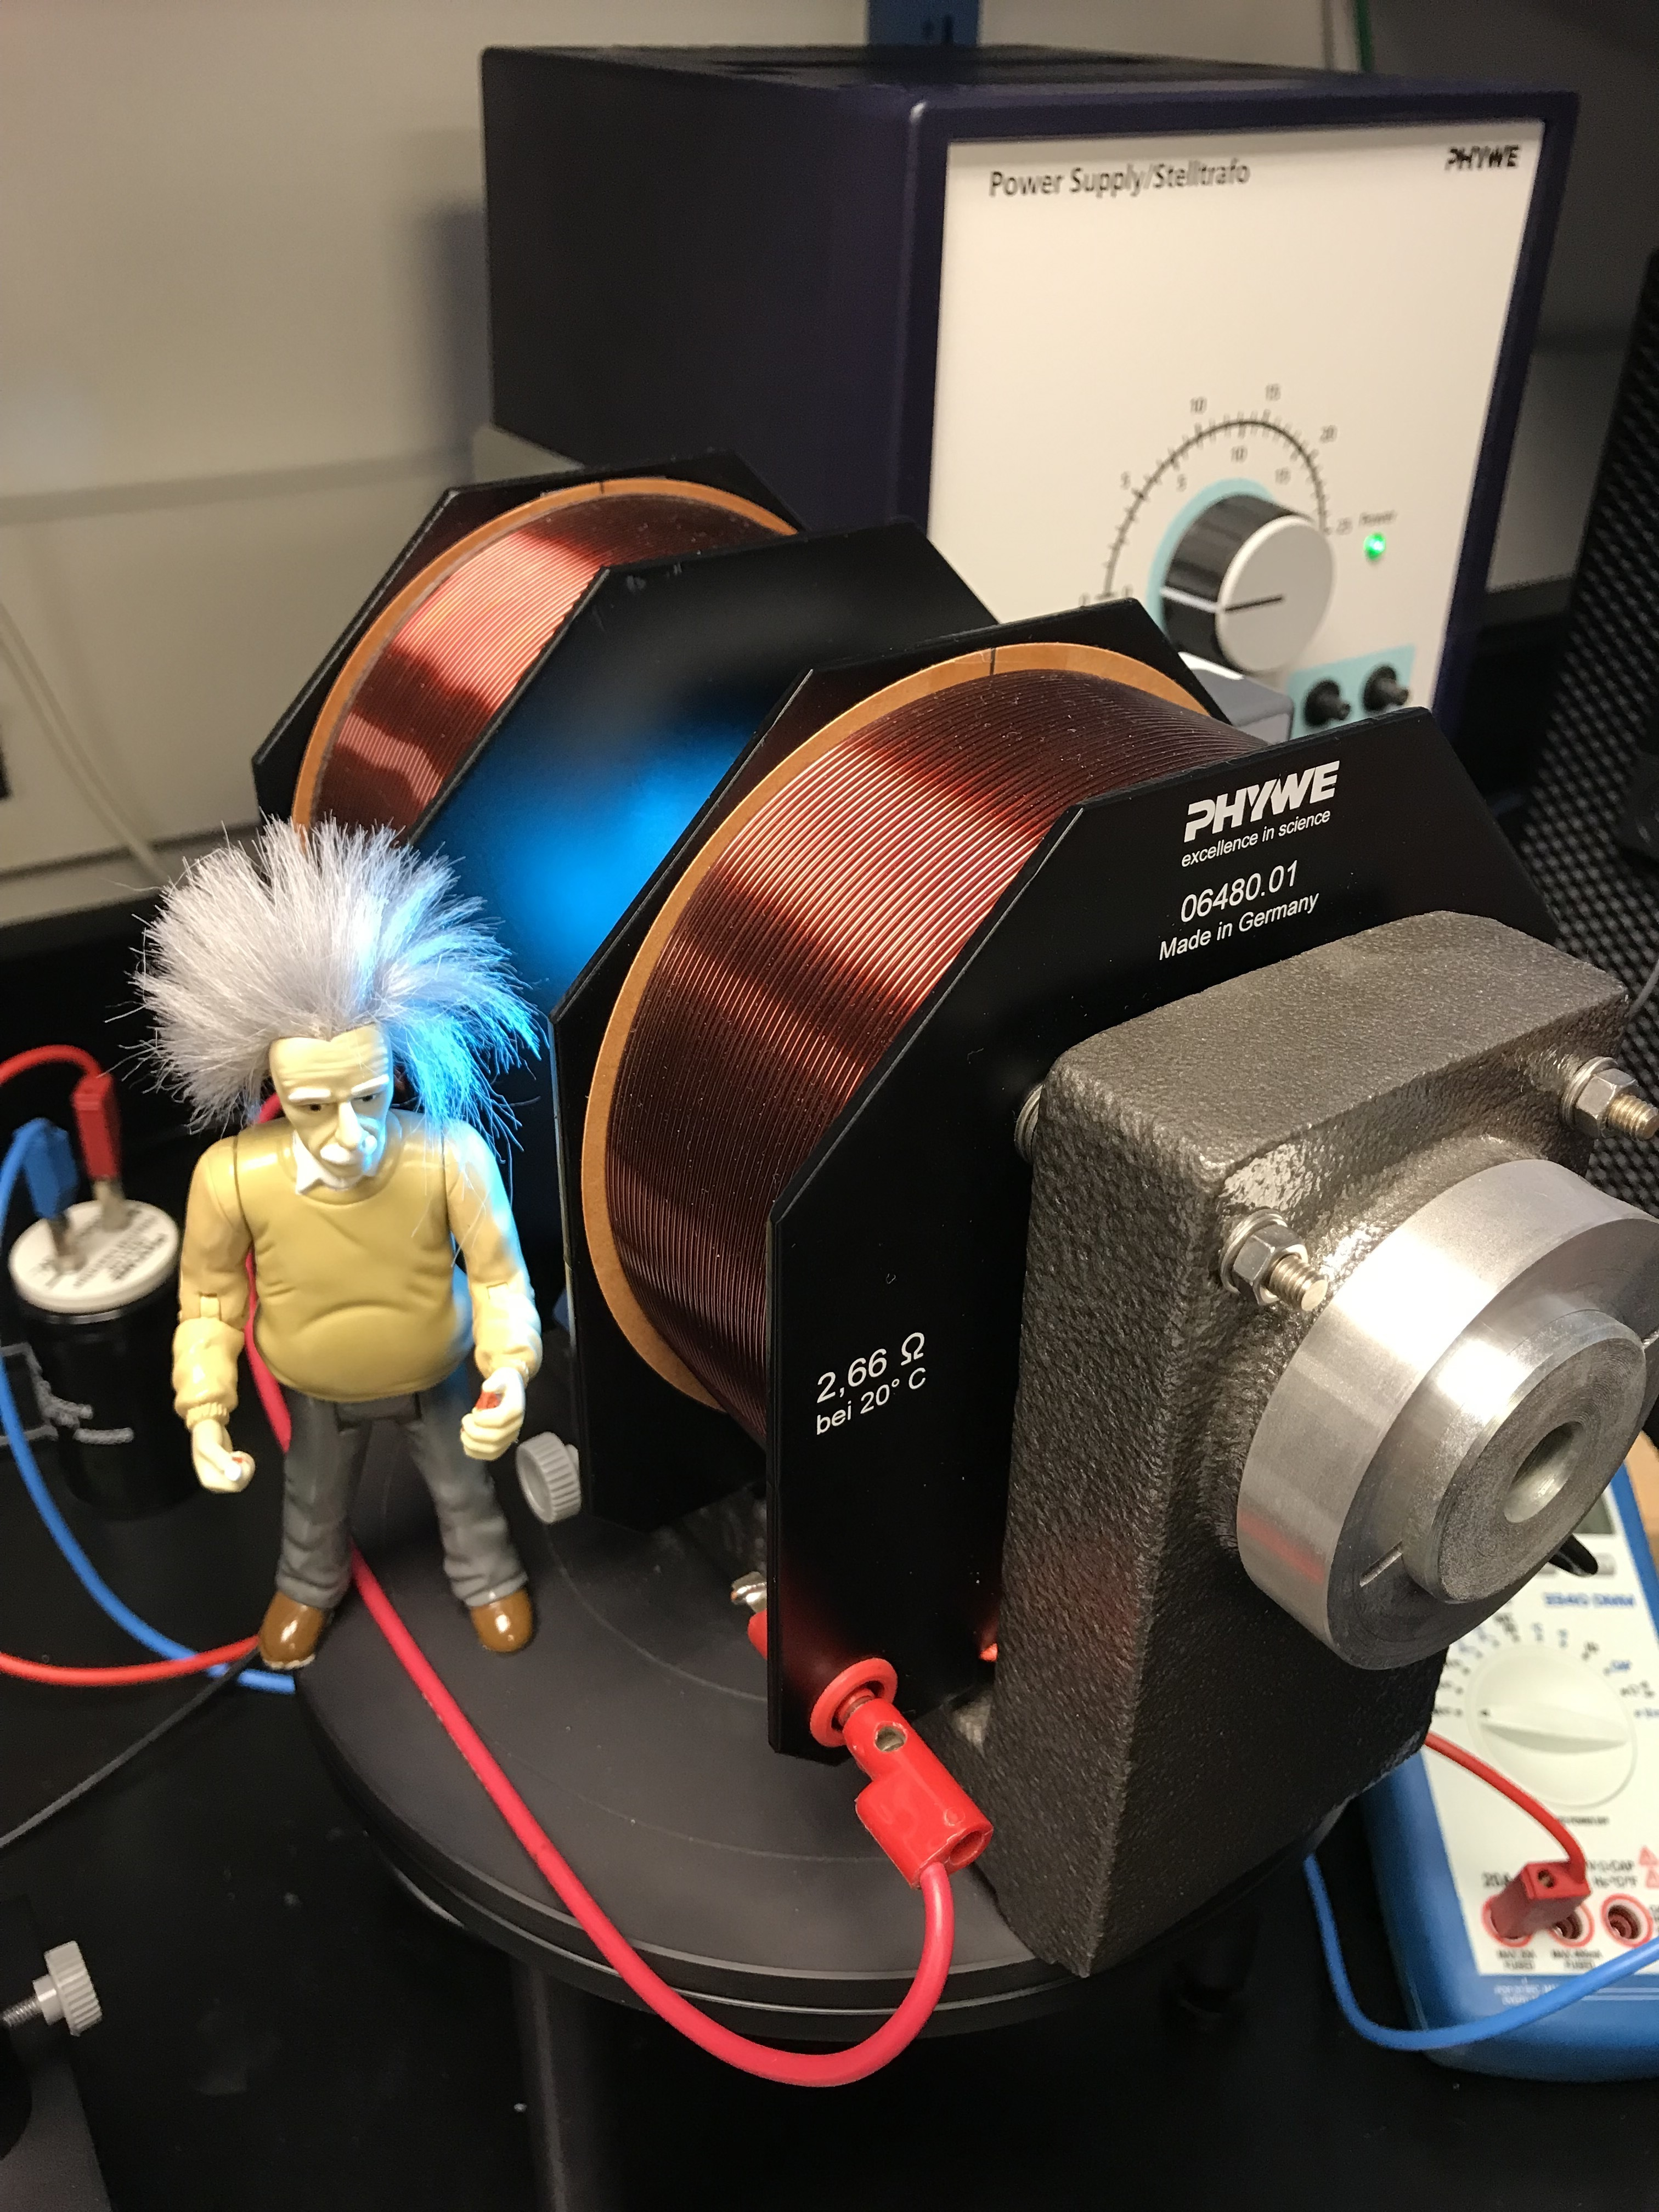
\includegraphics[height=10cm, width=10cm]{1.jpg}

  \vspace{20px}

  \textbf{II. Background Information}

  \vspace{10px}

  Magnetic fields effect how light behaves. The reason we study the Zeeman effect is that it has helped physicists to study the energy levels
  in atoms which is a very important topic in Quantum Physics.
  "In the late 1800s, Dutch physicist Pieter Zeeman made discovered that powerful magnetic currents would widen the convergences of units 
  of sodium under intense heat which is known is the Zeeman effect or \textbf{anomalous Zeeman effect}." \textcite{One}

  \vspace{20px}

  \textbf{I. Introduction}

  \vspace{10px}

  \textbf{III. Theory}

  \textbf{IV. Experimental Procedure}

  \textbf{V. Results}

  \textbf{VI. Discussion}

  \textbf{VII. Conclusions}

  \printbibliography
\end{document}